\documentclass{article}
\usepackage[utf8]{inputenc}
\usepackage[italian]{babel}
\usepackage[margin=1cm, top=1cm]{geometry}
\usepackage{graphicx}
\usepackage{makecell}
\pagenumbering{gobble}
\usepackage{float}

\usepackage{titlesec}
\titleformat{\section}{\LARGE\bfseries}{\thesection}{1em}{}

\title{\Huge{Constant Propagation}}
\date{}

\begin{document}
	
	\maketitle
	
	\section{Parametri}
	
	\begin{table}[h]
		\centering
		\Large
		\renewcommand{\arraystretch}{1.4}
		\begin{tabular}{|c|c|}
			\hline
			Domain &  \makecell{Insieme di coppie \\ $\textless variabile,\ valore\ costante\textgreater$} \\
			\hline
			Direction & \makecell[l]{Forward: \\ $out[B] = f_B(in[B])$ \\ $in[B] = \wedge\ out[pred(B)]$} \\
			\hline
			Transfer Function & $f_B(x)$ = $Gen_B \cup (x - Kill_B)$ \\
			\hline
			Meet Operation ($\wedge$) & Intersezione ($\cap$) \\
			\hline
			Boundary Condition & $out[EXIT] = \emptyset$ \\
			\hline
			Initial interior points & $out[B] = N$ \\
			\hline
		\end{tabular}
	\end{table}
	
	\vspace{1cm}
	
	\newpage
	
	\section{Iterazioni}
	
	\begin{table}[H]
		\centering
		\large
		\renewcommand{\arraystretch}{1.3}
		\begin{tabular}{|c|c|c|c|c|c|c|}
			\hline
			& \multicolumn{2}{c|}{\textbf{Iterazione 1}} & \multicolumn{2}{c|}{\textbf{Iterazione 2}} & \multicolumn{2}{c|}{\textbf{Iterazione 3}} \\
			\hline
			& IN[B] & OUT[B] & IN[B] & OUT[B] & IN[B] & OUT[B] \\
			\hline
			BB1 & $\emptyset$ & $\emptyset$ & $\emptyset$ & $\emptyset$ & $\emptyset$ & $\emptyset$ \\
			\hline
			BB2 & $\emptyset$ & $\textless k, 2\textgreater$ & $\emptyset$ & $\textless k, 2\textgreater$ & $\emptyset$ & $\textless k, 2\textgreater$ \\
			\hline
			BB3 & $\textless k, 2\textgreater$ & $\textless k, 2\textgreater$ & $\textless k, 2\textgreater$ & $\textless k, 2\textgreater$ & $\textless k, 2\textgreater$ & $\textless k, 2\textgreater$ \\
			\hline
			BB4 & $\textless k, 2\textgreater$ & \makecell{$\textless k, 2\textgreater$ \\ $\textless a, 4\textgreater$} & $\textless k, 2\textgreater$ & \makecell{$\textless k, 2\textgreater$ \\ $\textless a, 4\textgreater$} & $\textless k, 2\textgreater$ & \makecell{$\textless k, 2\textgreater$ \\ $\textless a, 4\textgreater$} \\
			\hline
			BB5 & \makecell{$\textless k, 2\textgreater$ \\ $\textless a, 4\textgreater$} & \makecell{$\textless k, 2\textgreater$ \\ $\textless a, 4\textgreater$ \\ $\textless x, 5\textgreater$} & \makecell{$\textless k, 2\textgreater$ \\ $\textless a, 4\textgreater$} & \makecell{$\textless k, 2\textgreater$ \\ $\textless a, 4\textgreater$ \\ $\textless x, 5\textgreater$} & \makecell{$\textless k, 2\textgreater$ \\ $\textless a, 4\textgreater$} & \makecell{$\textless k, 2\textgreater$ \\ $\textless a, 4\textgreater$ \\ $\textless x, 5\textgreater$} \\
			\hline
			BB6 & $\textless k, 2\textgreater$ & \makecell{$\textless k, 2\textgreater$ \\ $\textless a, 4\textgreater$} & $\textless k, 2\textgreater$ & \makecell{$\textless k, 2\textgreater$ \\ $\textless a, 4\textgreater$} & $\textless k, 2\textgreater$ & \makecell{$\textless k, 2\textgreater$ \\ $\textless a, 4\textgreater$} \\
			\hline
			BB7 & \makecell{$\textless k, 2\textgreater$ \\ $\textless a, 4\textgreater$} & \makecell{$\textless k, 2\textgreater$ \\ $\textless a, 4\textgreater$ \\ $\textless x, 8\textgreater$} & \makecell{$\textless k, 2\textgreater$ \\ $\textless a, 4\textgreater$} & \makecell{$\textless k, 2\textgreater$ \\ $\textless a, 4\textgreater$ \\ $\textless x, 8\textgreater$} & \makecell{$\textless k, 2\textgreater$ \\ $\textless a, 4\textgreater$} & \makecell{$\textless k, 2\textgreater$ \\ $\textless a, 4\textgreater$ \\ $\textless x, 8\textgreater$} \\
			\hline
			BB8 & \makecell{$\textless k, 2\textgreater$ \\ $\textless a, 4\textgreater$} & \makecell{$\textless k, 4\textgreater$ \\ $\textless a, 4\textgreater$} & \makecell{$\textless k, 2\textgreater$ \\ $\textless a, 4\textgreater$} & \makecell{$\textless k, 4\textgreater$ \\ $\textless a, 4\textgreater$} & \makecell{$\textless k, 2\textgreater$ \\ $\textless a, 4\textgreater$} & \makecell{$\textless k, 4\textgreater$ \\ $\textless a, 4\textgreater$} \\
			\hline
			BB9 & \makecell{$\textless k, 4\textgreater$ \\ $\textless a, 4\textgreater$} & \makecell{$\textless k, 4\textgreater$ \\ $\textless a, 4\textgreater$} & $\textless a, 4\textgreater$ & $\textless a, 4\textgreater$ & $\textless a, 4\textgreater$ & $\textless a, 4\textgreater$ \\
			\hline
			BB10 & \makecell{$\textless k, 4\textgreater$ \\ $\textless a, 4\textgreater$} & \makecell{$\textless k, 4\textgreater$ \\ $\textless a, 4\textgreater$ \\ $\textless b, 2\textgreater$} & $\textless a, 4\textgreater$ & \makecell{$\textless a, 4\textgreater$ \\ $\textless b, 2\textgreater$} & $\textless a, 4\textgreater$ & \makecell{$\textless a, 4\textgreater$ \\ $\textless b, 2\textgreater$} \\
			\hline
			BB11 & \makecell{$\textless k, 4\textgreater$ \\ $\textless a, 4\textgreater$ \\ $\textless b, 2\textgreater$} & \makecell{$\textless k, 4\textgreater$ \\ $\textless a, 4\textgreater$ \\ $\textless b, 2\textgreater$ \\ $\textless x, 8\textgreater$} & \makecell{$\textless a, 4\textgreater$ \\ $\textless b, 2\textgreater$} & \makecell{$\textless a, 4\textgreater$ \\ $\textless b, 2\textgreater$} & \makecell{$\textless a, 4\textgreater$ \\ $\textless b, 2\textgreater$} & \makecell{$\textless a, 4\textgreater$ \\ $\textless b, 2\textgreater$} \\
			\hline
			BB12 & \makecell{$\textless k, 4\textgreater$ \\ $\textless a, 4\textgreater$ \\ $\textless b, 2\textgreater$ \\ $\textless x, 8\textgreater$} & \makecell{$\textless k, 4\textgreater$ \\ $\textless a, 4\textgreater$ \\ $\textless b, 2\textgreater$ \\ $\textless x, 8\textgreater$ \\ $\textless y, 8\textgreater$} & \makecell{$\textless a, 4\textgreater$ \\ $\textless b, 2\textgreater$} & \makecell{$\textless a, 4\textgreater$ \\ $\textless b, 2\textgreater$ \\ $\textless y, 8\textgreater$} & \makecell{$\textless a, 4\textgreater$ \\ $\textless b, 2\textgreater$} & \makecell{$\textless a, 4\textgreater$ \\ $\textless b, 2\textgreater$ \\ $\textless y, 8\textgreater$} \\
			\hline
			BB13 & \makecell{$\textless k, 4\textgreater$ \\ $\textless a, 4\textgreater$ \\ $\textless b, 2\textgreater$ \\ $\textless x, 8\textgreater$ \\ $\textless y, 8\textgreater$} & \makecell{$\textless k, 5\textgreater$ \\ $\textless a, 4\textgreater$ \\ $\textless b, 2\textgreater$ \\ $\textless x, 8\textgreater$ \\ $\textless y, 8\textgreater$} & \makecell{$\textless a, 4\textgreater$ \\ $\textless b, 2\textgreater$ \\ $\textless y, 8\textgreater$} & \makecell{$\textless a, 4\textgreater$ \\ $\textless b, 2\textgreater$ \\ $\textless y, 8\textgreater$} & \makecell{$\textless a, 4\textgreater$ \\ $\textless b, 2\textgreater$ \\ $\textless y, 8\textgreater$} & \makecell{$\textless a, 4\textgreater$ \\ $\textless b, 2\textgreater$ \\ $\textless y, 8\textgreater$} \\
			\hline
			BB14 & \makecell{$\textless k, 4\textgreater$ \\ $\textless a, 4\textgreater$} & \makecell{$\textless k, 4\textgreater$ \\ $\textless a, 4\textgreater$} & $\textless a, 4\textgreater$ & $\textless a, 4\textgreater$ & $\textless a, 4\textgreater$ & $\textless a, 4\textgreater$ \\
			\hline
			BB15 & \makecell{$\textless k, 4\textgreater$ \\ $\textless a, 4\textgreater$} &  $\emptyset$ & $\textless a, 4\textgreater$ & $\emptyset$ & $\textless a, 4\textgreater$ & $\emptyset$ \\
			\hline
		\end{tabular}
	\end{table}
	
	\begin{figure}[h]
	\centering
	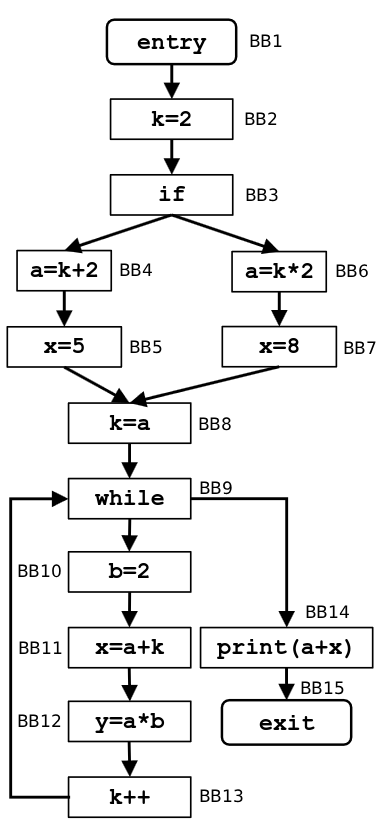
\includegraphics[height=15cm]{img/CFG.png}
	\caption{CFG}
	\end{figure}
	
\end{document}